% !TeX document-id = {e96318ba-ee8c-4009-b5ac-484871d58952}
% !TeX encoding = UTF-8
% !TeX program = pdflatex
% !BIB program = bibtex

%%% Um einen Artikel auf deutsch zu schreiben, genügt es die Klasse ohne
%%% Parameter zu laden.



\documentclass[english]{lni}
%%% To write an article in English, please use the option ``english'' in order
%%% to get the correct hyphenation patterns and terms.
%%% \documentclass[english]{class}
%%
\usepackage{xspace}
\usepackage[utf8]{inputenc}
\usepackage{xcolor}
\usepackage{authblk}
\definecolor{backcolour}{rgb}{0.95,0.95,0.92}
\begin{document}

\title[Precision Farming]{Precision Farming}
\author[]{Tunde Oluwayemi Aluko\footnote{ \email{tunde-oluwayemi.aluko@stud.hshl.de}}}

\author[]{Enkeledi Mema\footnote{ \email{enkeledi.mema@stud.hshl.de}}}

\author[]{Fawad Murad\footnote{
\email{fawad.murad@stud.hshl.de}}}

\author[]{Muhammad Moaz Amin\footnote{
\email{muhammad-moaz.amin@stud.hshl.de}}}
\affil[]{Department of Electronic Engineering, Hamm-Lippstadt University of Applied Sciences}



\startpage{1} % Beginn der Seitenzählung für diesen Beitrag / Start page
\booktitle{ Autonomous Lab} % Name of book title
\year{Winter Term 2021}

\maketitle
\tableofcontents
\begin{abstract}
(Fawad Murad) \\

The idea of precision farming is to apply inputs into production (such as chemicals, seed and fertilizer) only when and where it is needed for the most cost-effective production. Basically, it provides a framework through which farmers can better understand and regulate what occurs on their fields. In this documentation, it is demonstrated that how different aspects of precision farming work and how we can get an idea of improvement in several places like how well we can train our system for better classification of different crops or detecting the problems using drones and the high-resolution map produced by internal system. Thus, the goal is how new technology now make it possible to put precision farming into practice in a real-world context in order to minimize costs and maximize benefits for increasing agricultural producing units' economic return.



\end{abstract}

\newpage

\newpage

\section{Introduction And Motivation (Tunde Oluwayemi Aluko)} 

According to the United Nations\cite{united2019department}, the world population will increase by 2 billion in 2050. To meet the ever-increasing population’s food demand, farmers need to maximise their productions. In order to maximise production, precision farming is the future farming system that farmers need to adopt. Precision farming improves efficiency, productivity and cost.

Bahr et al.\cite{bahr2015eip} defines precision farming as a farming system that focuses on monitoring plants, animals and fields in real-time and provides responses. Precision farming often employs robotic systems like Unmanned Aerial Vehicles(UAV) to continuously observe and treat any part of the farm field or crops with its precise needs\cite{razaak2019integrated}. These concepts improve farming productivity by optimising the inputs process, reducing labour cost, and increasing crop yield.

In this project, we have used the cyber-physical system (CPS) concept combined with deep learning algorithms to design and implement a precision farming prototype.

We first discuss our design approach by analyzing the system, after which we propose an architecture, then interpret our concept using use-case diagrams. We proceed to model our design concept in Petri-net with the aid of TAPAAL software as a support tool and use fastai\cite{howard2020fastai}, a deep learning framework built on PyTorch to model and train our deep learning algorithm. Our focus area of precision farming is weed detection.

\section{Analysis of the System (Enkeledi Mema)}
Precision farming (PF) is perceived as a system which goal is to increase the productivity by minimizing the resources. Usually there are different operation that occur in PF. After further requirements analyses, it is possible to split these operations in three main categories. The first is operation relates to the exploration. The second it associated with monitoring results. The last operation is to develop some strategies for field treatment. All these operation will be performed mainly by drones and partially from vehicles on terrain. Therefor, it is useful to build different use case based in specific scenarios. The first scenario is surveillance operation which is performed by a specific drone. These drones are called monitoring drones. The next scenario that needs to be taken in consideration is autonomously driving agricultural vehicles on terrain. During the work distribution, one drone might not be sufficient to fulfill an operation.

\begin{figure}[h]
    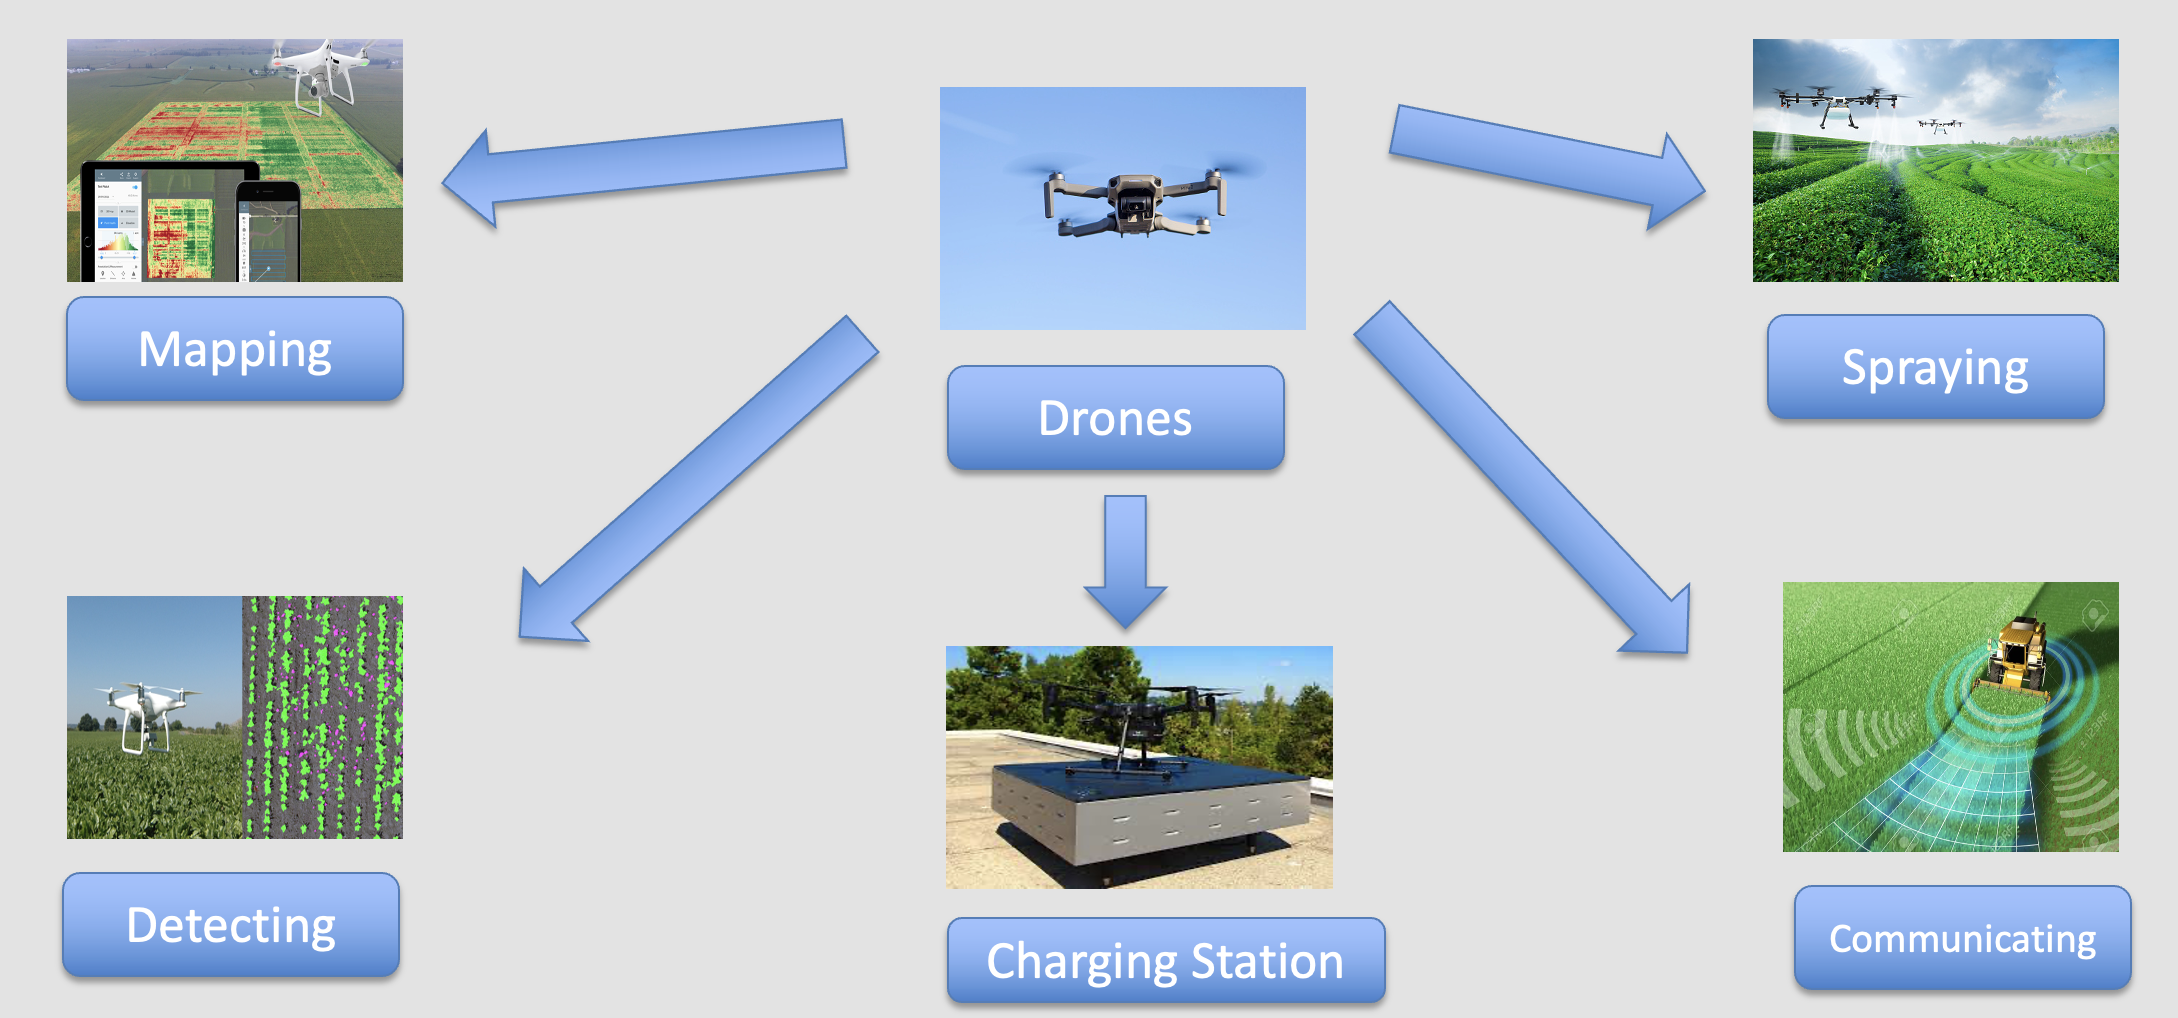
\includegraphics[width=.9\textwidth]{Template/fig/fig5.png}
    \centering
    \caption{Precision Farming System.}
\end{figure} 
Therefore, several drones operations scenario is taken in consideration. To have a better control and information for the holistic system external system scenarios are beneficial\cite{article}.
\subsection{Use Case}
\subsubsection{Use Case for Monitor  and Control of the Holistic System
(Enkeledi Mema)}
Based on the scenario for overall system monitoring the following use case diagram is generated.The purpose of this use case is to analyse and make visible all component of the system . Also external systems are included.
\begin{figure}[h]
    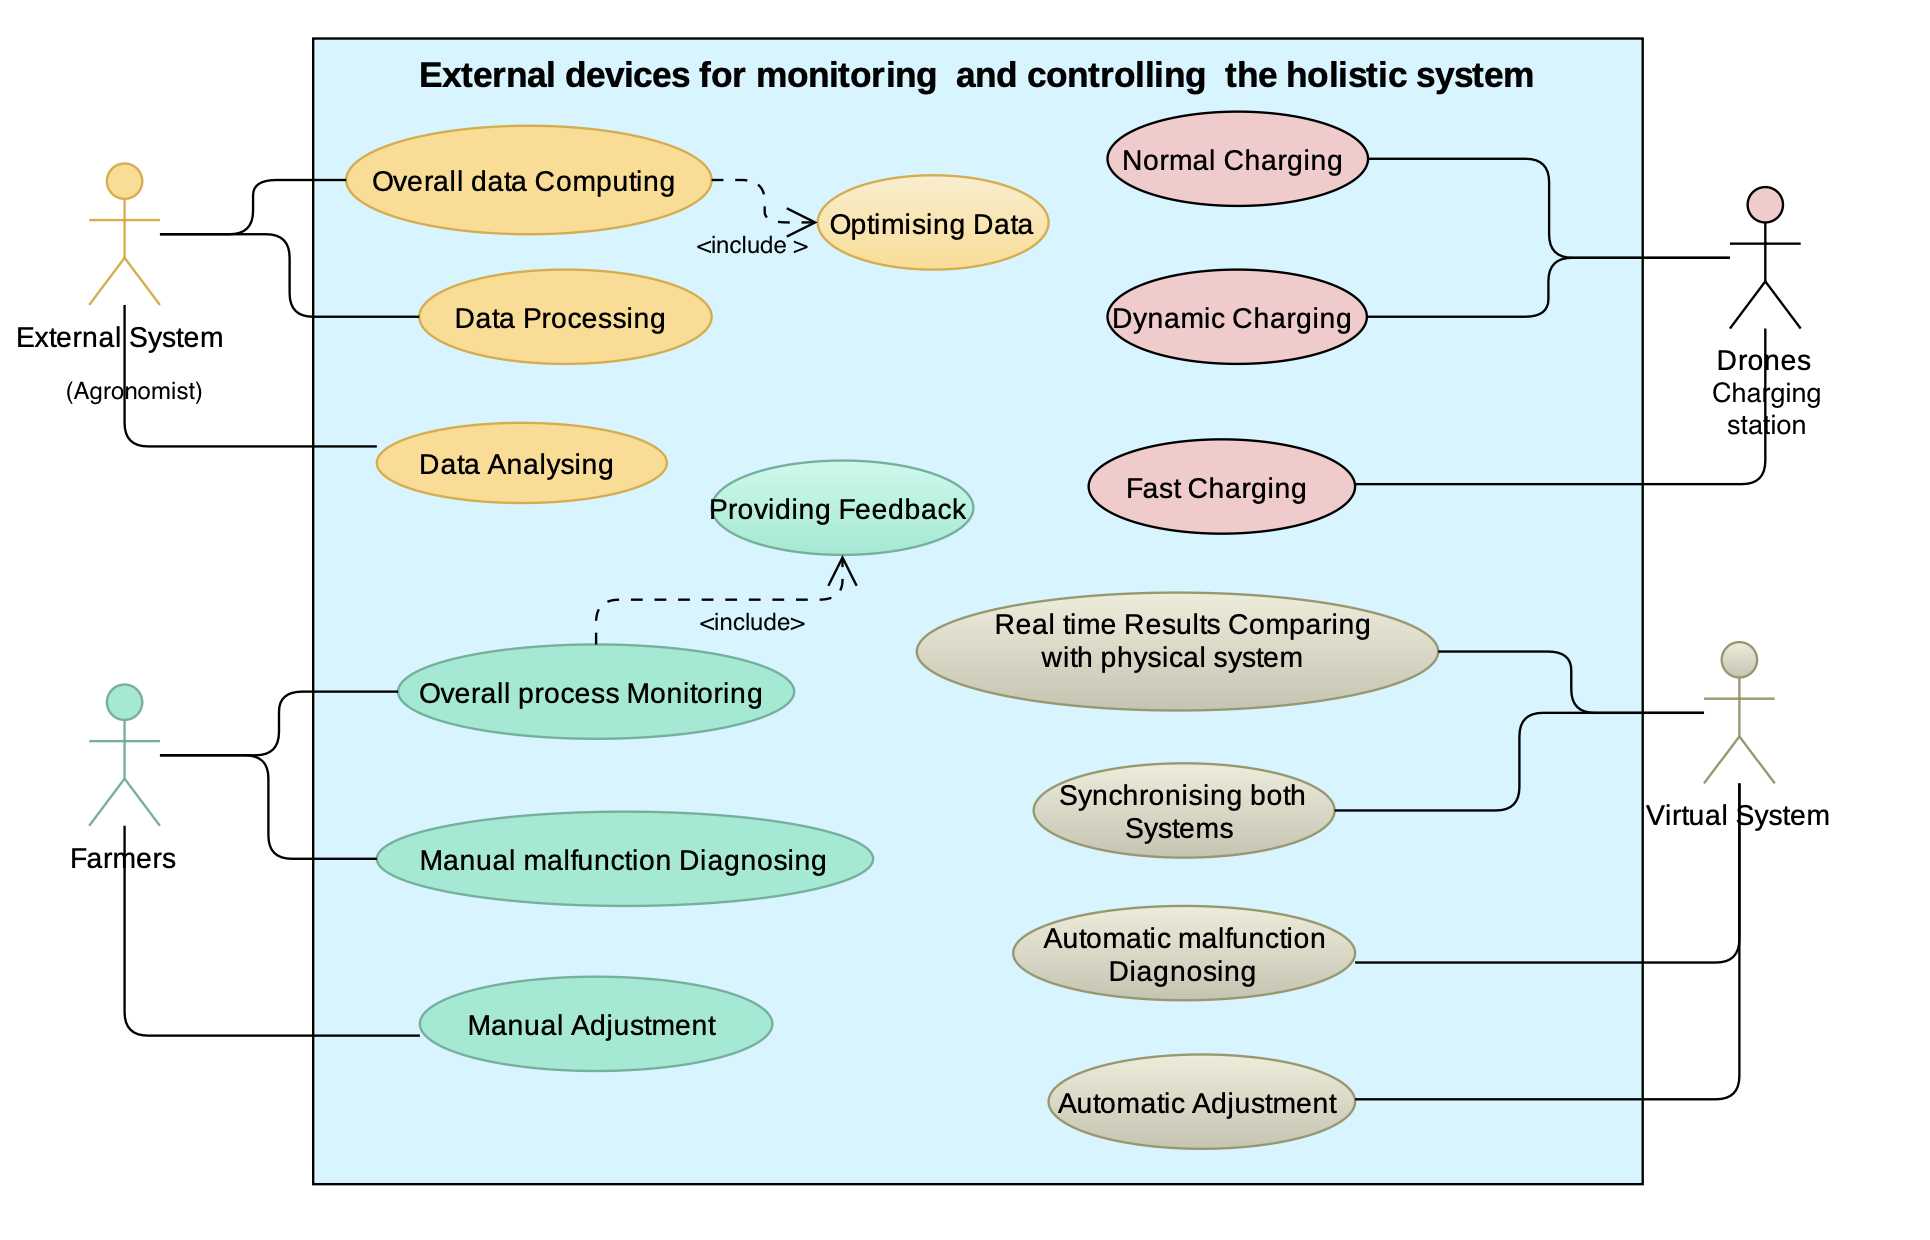
\includegraphics[width=.9\textwidth]{Template/fig/fig1.png}
    \centering
    \caption{Use Case of the Holistic System.}
\end{figure} 
In this use case is presented the communication that happens in between different actors.The first actor that has access to the system is the farmer. As it is shown in the use case the farmer can monitor the overall process.The farmer also can access the system and can perform manual adjustment. The other actor is an external system that can control the environment. This external system might be a person for example an agronomist. In the same time might be an institution or company that is interested in specific or partial information.This includes data processing or data computing.The next actor is a virtual system that provides the simulation in real time how the system is performing . Usually the virtual system compares the date in real time with the physical system. In case of a malfunctions it can generates alerts and provide information for the error that might occur.The next and last actor is the  autonomous charging station.The charging station communicate directly to the drones.It can provides a dynamic charging for the drones based on specific priorities.



\\
\newpage
\subsubsection{Use Case Specification of Monitoring by Drone  (Fawad Murad)} 
In this scenario, we have the following actors and their use cases:
\begin{itemize}
    \item Drone: (i) The first use case or goal of the drone in this scenario is to take several images by multispectral camera. (ii) The second use case of it is to record the imagery data.
    \item Internal System: (i) Internal system will overlap the pictures once the data is recorded by drone (ii) and then it will produce a high-resolution map of health of entire field (i.e 2400 times more detailed than satellite imagery).
    \item Farmer: (i) The first service of the farmer comes in the very beginning of this context and i.e. to set up drone path over the field to be mapped. (ii) to look into map using reflectance property (iii) Once the HD-Map is produced by internal system, then it will observe how well plants are reflecting the light from the Sun (iv) and another responsibility of the farmer comes at the end i.e. to use the analyzed information from Agronomist for the better growth. Like when and where to apply fertilizer or pesticide or how to manage irrigation.
    \item Agronomist: (i) The first use case of Agronomist is to scout and take samples of plant and soil (from the areas that are under some kind of stress) using drone data (ii) then analyse the samples. (iii) Once the samples are examined, it will inform the farmer about the analysis.
\end{itemize} 
\begin{figure}
    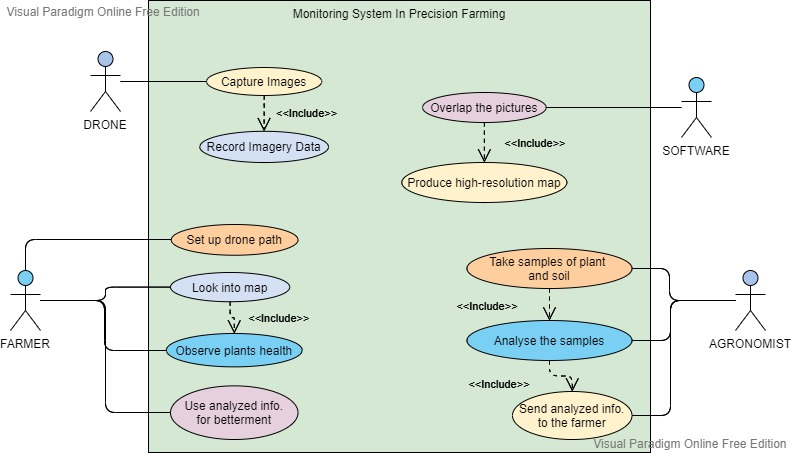
\includegraphics[width=1\textwidth]{Template/fig/Monitoring System in Precision Farming.jpg}
    \centering
    \caption{Monitoring System in Precision Farming}
\end{figure} 

MAP DETAILS: 
These maps give us an early warning and allow us to solve the problems: \\
(i) plants in green areas of map are extremely healthy  (ii) plants in red areas of map are facing serious issues like drainage problems, pest infestation,etc.  (iii) plants in yellow-orange areas of map are suffering unhealthiness from early stage which human   eye cannot identify that easy.



\subsubsection{Use Case: Multiple Drones (Tunde Oluwayemi Aluko)}
\begin{figure}[htp]
    \centering
    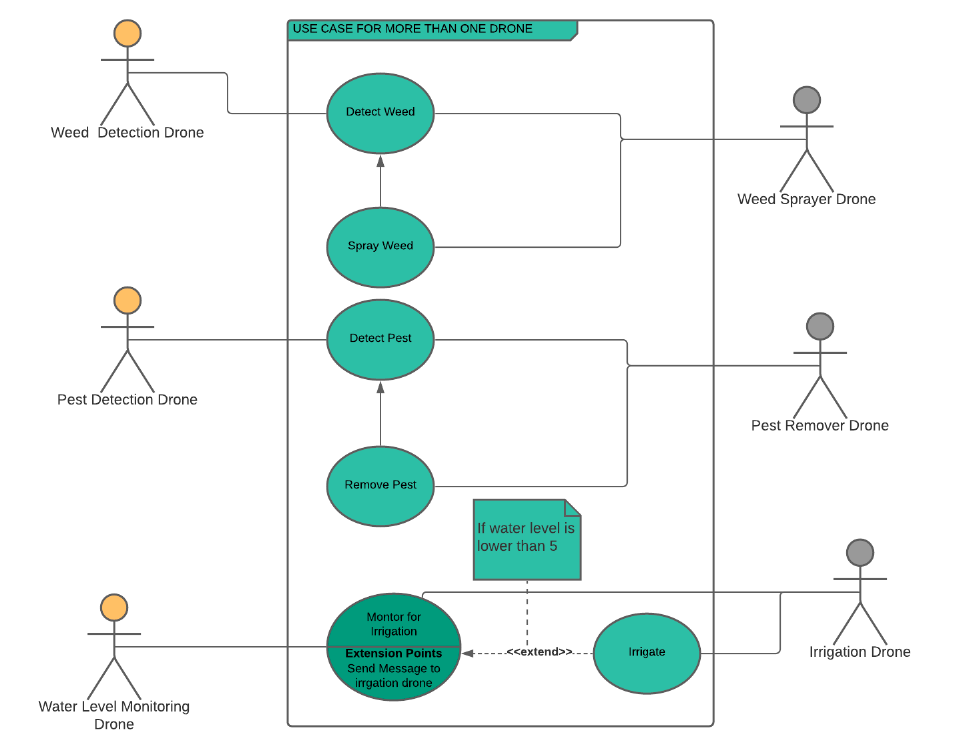
\includegraphics[height=5cm]{Template/fig/multiple_drone_usecase.png}
    \caption{Use-Case Diagram for Multiple Drones}
    \label{fig:multilpe_drones}
\end{figure}

A single drone has been used in many aspects of precision farming,
such as spraying or monitoring extensive farmland; however if the farmland is a bit larger, it can be inefficient because it requires considerable time and energy. In contrast,
when using multiple drone systems, it is possible to carry out cooperative
works simultaneously (collaboration) or individual agricultural tasks on the assigned farmland (a division of labour).

Figure \ref{fig:multilpe_drones} describes the use-case diagram where we have six drones; weed detection drone works in collaboration with the weed sprayer drone. The same concept goes for the pest detection drone and the pest remover drone.

\subsubsection{Use Case Specification of Autonomous Farming Vehicles (Moaz)}
In this scenario the autonomous farming vehicles will carry out the farming operation of harvesting the crop and if there is some hindrance in the path obstacle avoidance manoeuvre will be carried out. In this scenario we have the following actors and their use cases. Figure 4 shows the Use Case diagram for this scenario. 

\begin{itemize}
    \item \textbf{Farming Vehicle:} Farming robot is the most important actor of this scenario and it is going to perform the on ground operation of farming and is also going to drive autonomously on the provided path data. The  motor of farming vehicle which is responsible for the mobility of the vehicle is actuator without which the whole operation will fail as vehicle will not be able to move.
    
    \item \textbf{Farming Scientist:} The role of the scientist is to carry out manual operation of the farming vehicle in case there is a situation where autonomous driving is deactivated or is not accessible then farming scientist is going to operate the vehicle remotely. Farming scientist is also the one who is going to provide the plant information to the vehicles so harvesting operation is carried out and all the pests are removed in time so the main crop is saved. One other role of the scientist is to provide route data which along with the present drone data is fed to the robot so it can start moving. The scientist defines the boundaries which the robot cannot cross and will automatically turn off if breached.

    
    \item \textbf{Drones-Routing:} These are the drones which are collecting data that is required to map out the whole field. This data is updated in real time through wireless capabilities. These drones follow the trajectory of the vehicle and they also follow which driving path is taken by the vehicle. The drones also send back the data to the scientist so he can monitor any errors present in the autonomous operation.
    
    \item \textbf{Operational-Drones} (i) While the vehicle is moving around the field, Operational-Drones are acting as the vehicle's eyes. They are capturing high resolution images so that they can be compared with the algorithm present which will allow the harvesting operation to be carried out. (ii) These Drones also allow the farming vehicle to detect which plant is to be harvested and which is to be left aside as it has not yet fully bloomed.  The secondary role of these images is to update the data-set currently present so the complete process of reaping the crop has minimal errors. (iii) As multiple vehicles and other unforeseen obstacles can be present in field at any given time, Operational-Drones detect that and send the signal to the farming robot so that it can execute the obstacle avoidance manoeuvre. 
  
\end{itemize}
\begin{figure}[h]
    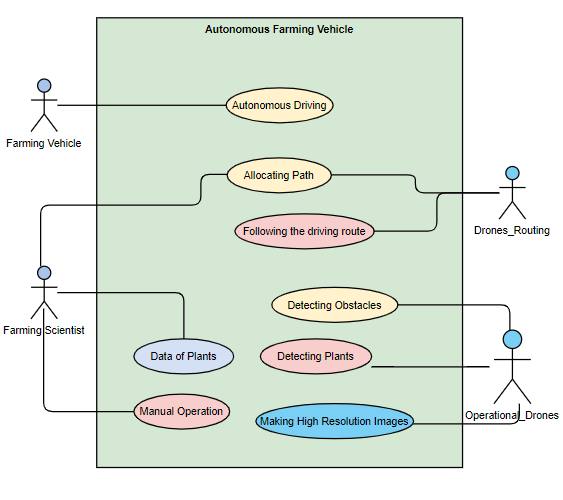
\includegraphics[width=.65\textwidth]{Template/fig/fig 5.png}
    \centering
    \caption{Autonomously driving Farming vehicles}
\end{figure}
\subsection{ System Architecture (Enkeledi Mema)}
Based on requirements and specifications that were achieved through use cases and scenarios,the overall system architecture was developed.
\begin{figure}[h]
    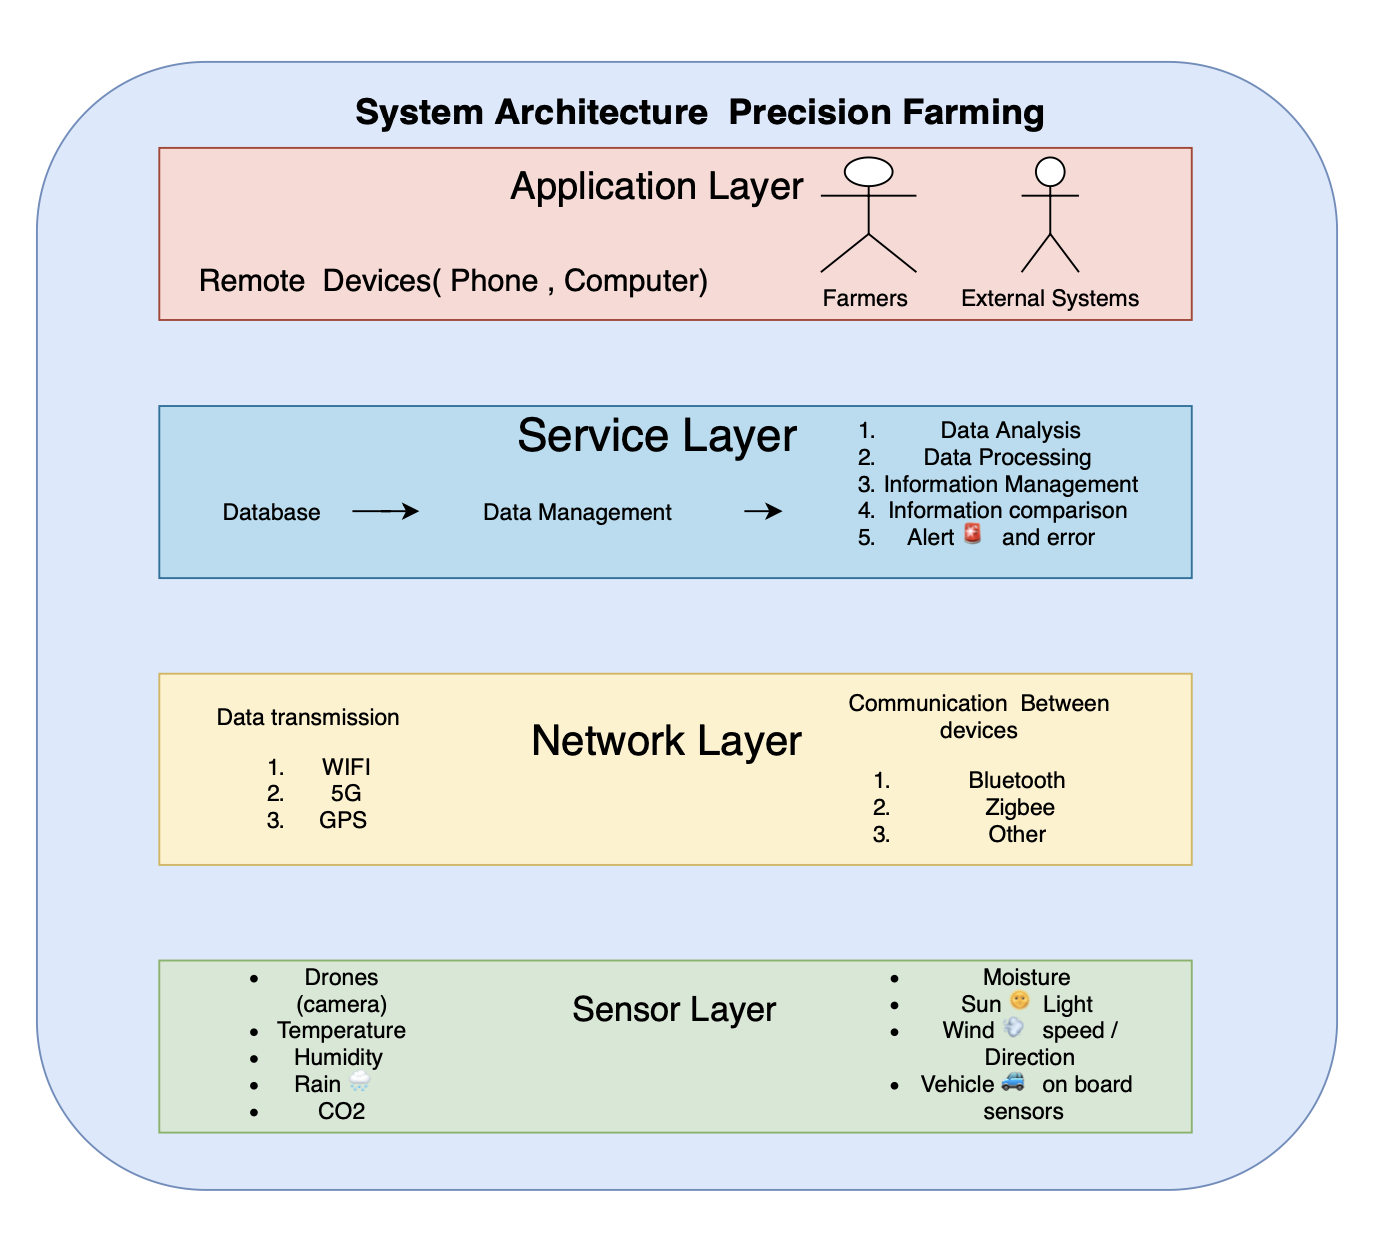
\includegraphics[width=.9\textwidth]{Template/fig/fig2.png}
    \centering
    \caption{ System Architecture.}
\end{figure} 
\begin{itemize}
    \item Sensor layer is  the first basic layer. In this layer are included all the types of sensor that are required to develop the precision farming.The sensors are in a wide verity depending on the purpose of usage.But it is possible to slit in terrain sensors that monitor the soil parameters and other conditions. The second group is the sensors used in different autonomous vehicles.
    \item The next layer is the network layer.This layer is responsible for all communication behaviours. The communication can be separated in long range data transitions and communication between devices.For data transmission it is possible to use WiFi, 5G etc. For communication between devices it is possible to use Bluetooth, Zigbee etc. This layer is considered as a bridge for upcoming layers
    \item The Upcoming layer is the service layer. This layer is responsible for all data set manipulation.With other words  in this layer are performed data management.In it is included data processing and analysing as well. Furthermore errors and alerts are part of this layer.It assist to switch to the next above layer. 
    \item The final and top layer is application layer.This layer is responsible for granting access.Remote devices are included as well. A farmer or external system(Agronomist) can communicate with the system through this layer. Usually the application layer is responsible for input and output information for the system.
\end{itemize} 

\section{Modelling and Verification  (Fawad Murad)}

We used TAPAAL for modelling and verifying our Timed-Arc Petri Nets in order to have a better illustration of how precision farming thoroughly works. 
A graphical editor for developing TAPN models, a simulator for experimenting with the built nets, and a verification environment that automatically answers logical inquiries expressed in a subset of CTL logic (EF, EG, AF, AG) are all included in the TAPAAL tool. TAPAAL has the ability to check/verify model-related queries. There are a lot of options in the query dialog. To begin, you can give your query a name at the very top of the window. TAPAAL will convert your model to a Network of Timed Automata (NTA) and then utilize the UPPAAL verification engine on the resulting NTA to accomplish the actual verification. 

\subsection{Overall Communication Implemented in TAPAAL(Enkeledi Mema)}

Based on the use case for the holistic system,the next step is to model the system.To activate the communication the cloud based system should be activated and some requests from a farmer or an external system have arrived.Depending on the type of request, we can receive  different information regarding the drone status,vehicles on terrain status and sensors on the field.In case of the drones status there is a shared transition with multiple drones TAPAAL model as it is shown in the picture. After the Information is received the farmer can check the status and for any type of malfunction. In case of such errors he can make manual adjustments based on conditions.
\begin{figure}[h]
    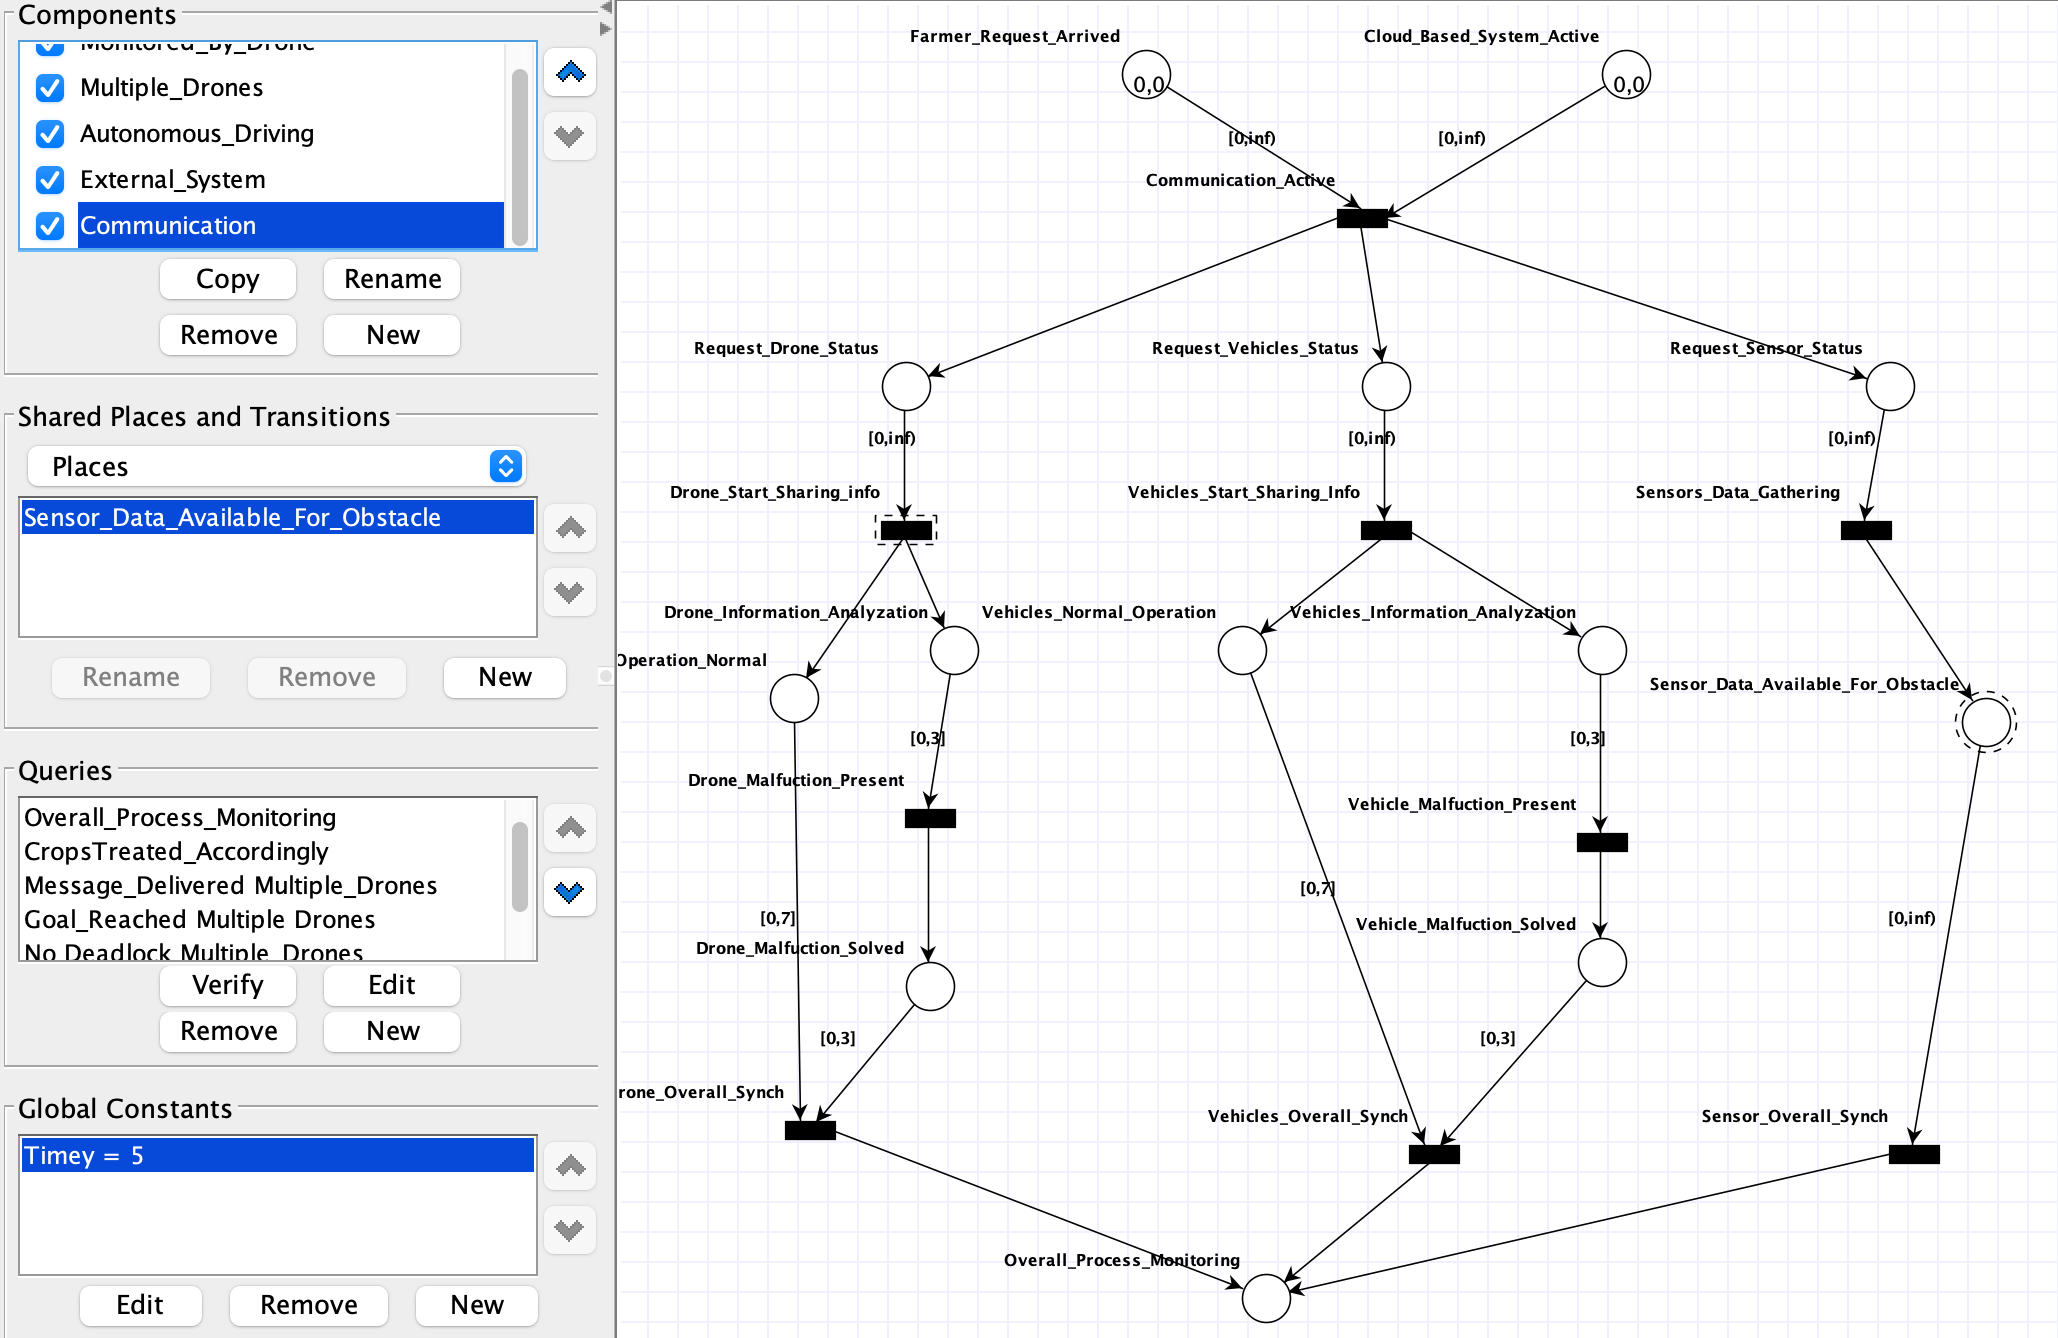
\includegraphics[width=.9\textwidth]{Template/fig/fig3.png}
    \centering
    \caption{ Overall Communication Modelling and Verification. }
\end{figure}
In the same way the farmers can check the status of the autonomous vehicles on the field. In case of malfunction the can analyse and solve the malfunctions manually. The same scenario applies to sensors in the field.In this case there is a shared place with autonomous driving TAPAAL model.The farmer has access to the sensors and in case of malfunction it is possible to make adjustments or calibration manually. 

\subsubsection{External System for Charging Station(Enkeledi Mema) }
As an external system,the smart charging station is modelled. First of all the smart charging stations should be running and waiting for drones requests. Drones can communicate directly with the charging station in case they need to be recharged. In case of an incoming drone request the smart station check if the station is available.If the station is available ,for the drone is assigned a time slot. This process is dynamic. This means that the queue is decided based on the priorities and can be updated.The next step is to allocate a time slot for charging. After the charging is done ,the drone is able to fly over the field again. This model shares the same charging done transition with multiple drone TAPAAL model.After the charging process is finished the queue is updated. Regarding the new incoming request new priorities are placed.The process can be repeated and the charging station is capable to operate autonomously. 
\begin{figure}[h]
    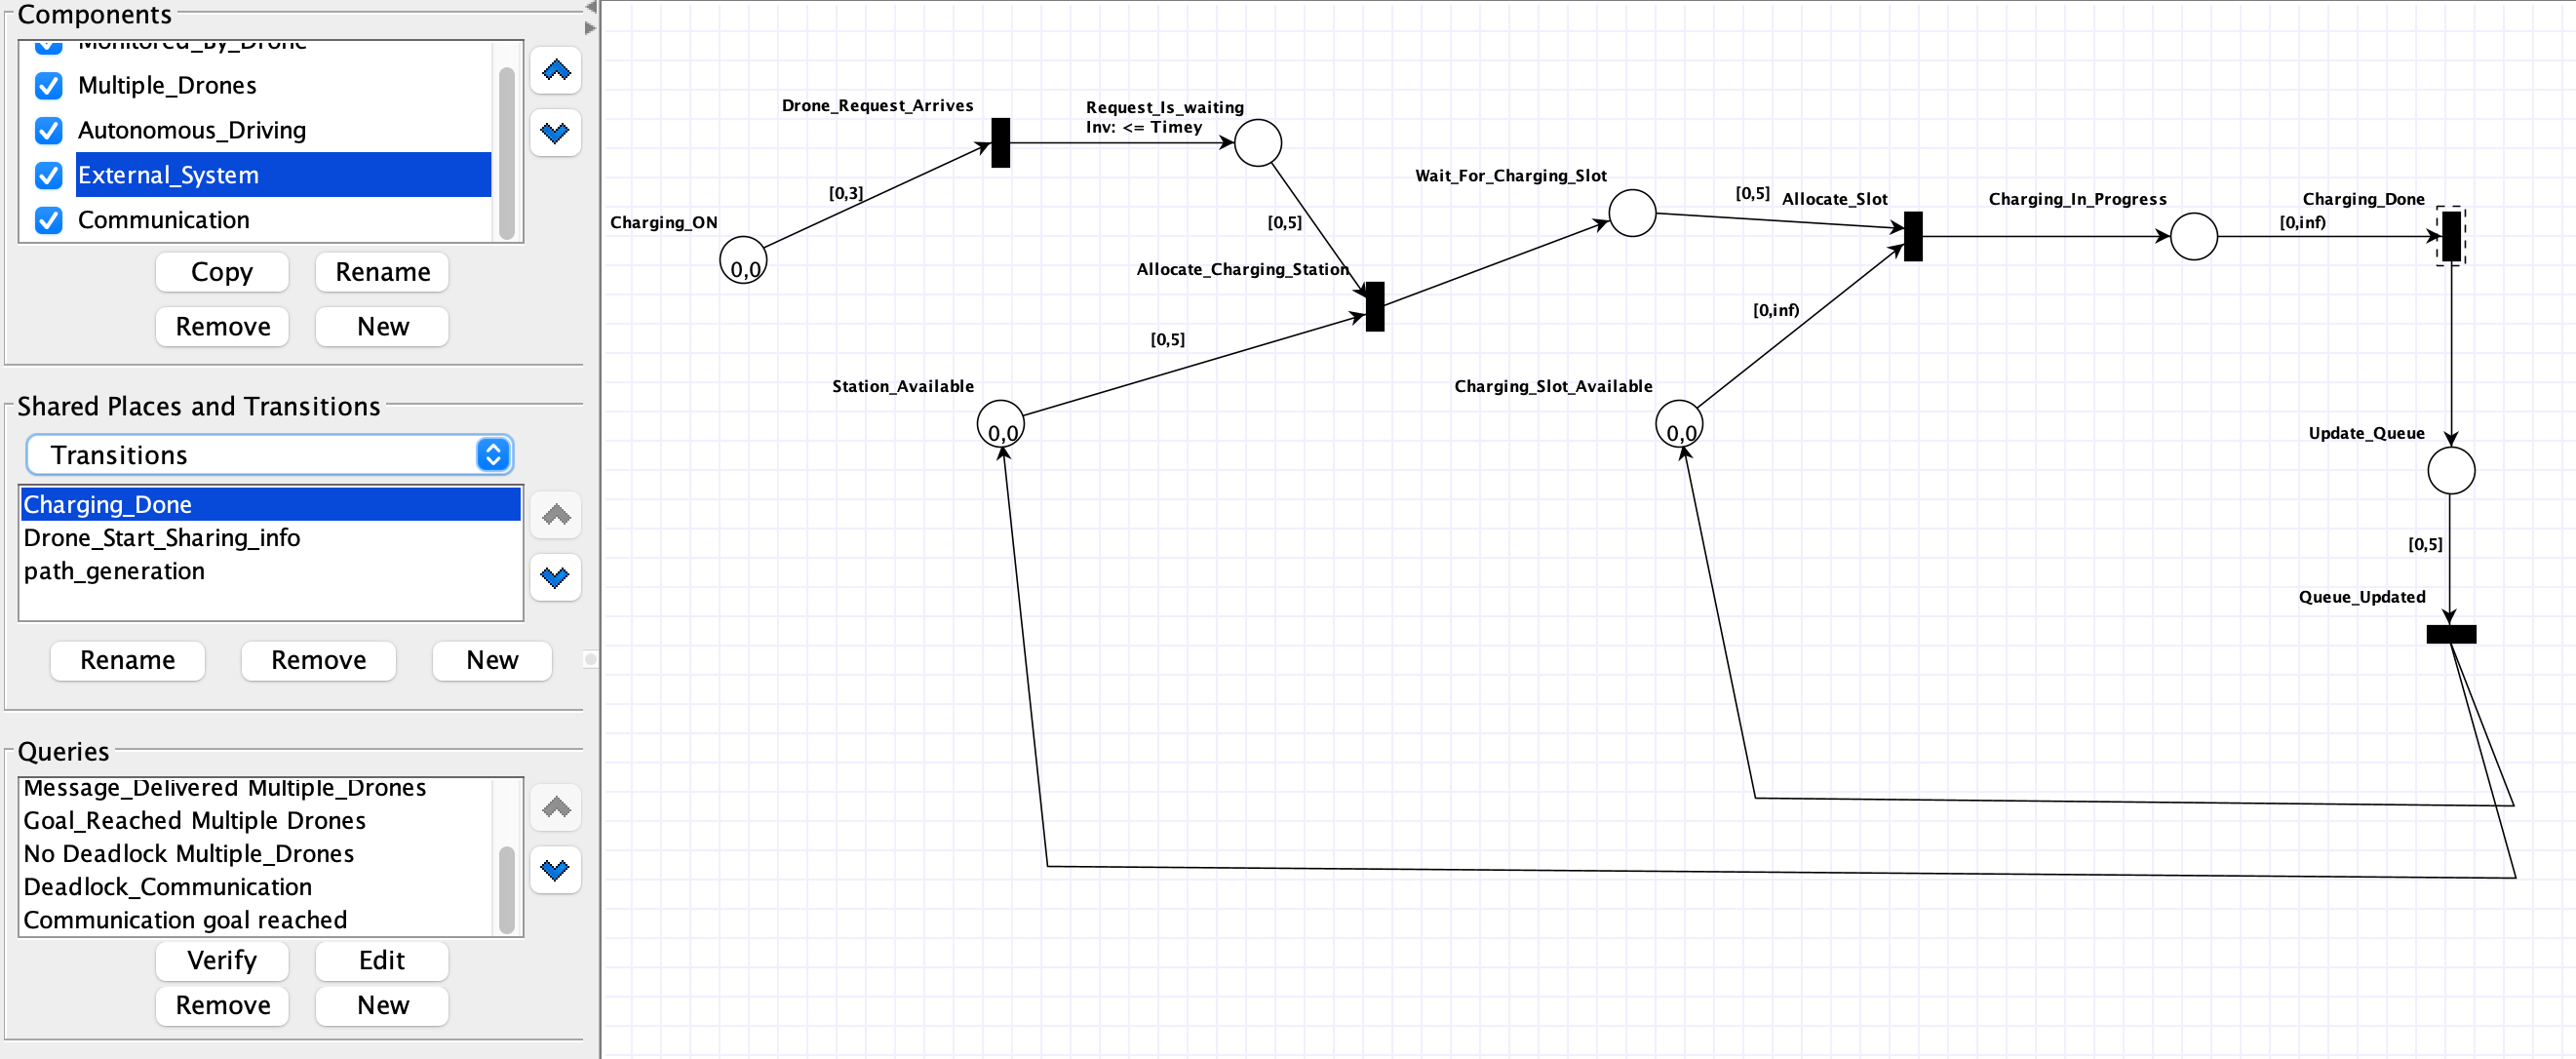
\includegraphics[width=.9\textwidth]{Template/fig/fig4.png}
    \centering
    \caption{ External System (Charging Station) Modelling and Verification .}
\end{figure}

\subsubsection{TAPAAL Models Verification (Enkeledi Mema) }
The next step after modelling is verifying. Verification are very important because they  ensure the system functionality,reliability and safety.In both TAPAAL models is verified if there are any deadlock. Due to analysing phase is proofed that the models do not contain any deadlock that might compromise the system behaviour.In the external system model it is important to check if a specific transition or place is reached.This type of verification is done for the charging done state in the external system.By using the same approach it is checked if the communication is reached. Another verification regarding the overall system monitoring is performed as it is shown in the pictures. 



\subsection{Tapaal Model of Monitoring by Drone  (Fawad Murad)}

In the beginning of this scenario, the drone path is given by the farmer. This path contains the information of the area of field to be monitored. Once the path is introduced, the next place in this model is for capturing images, in which the drone is capturing the photos of that specified area and recording the data of those images. The next place is for the generation of high-resolution map/path which is done by the internal system or software. After this place, there comes a transition where the information of that path is shared with one of the places in another interlinked scenario “Autonomous Driving” because that information is used in further places of that scenario.

\begin{figure}
    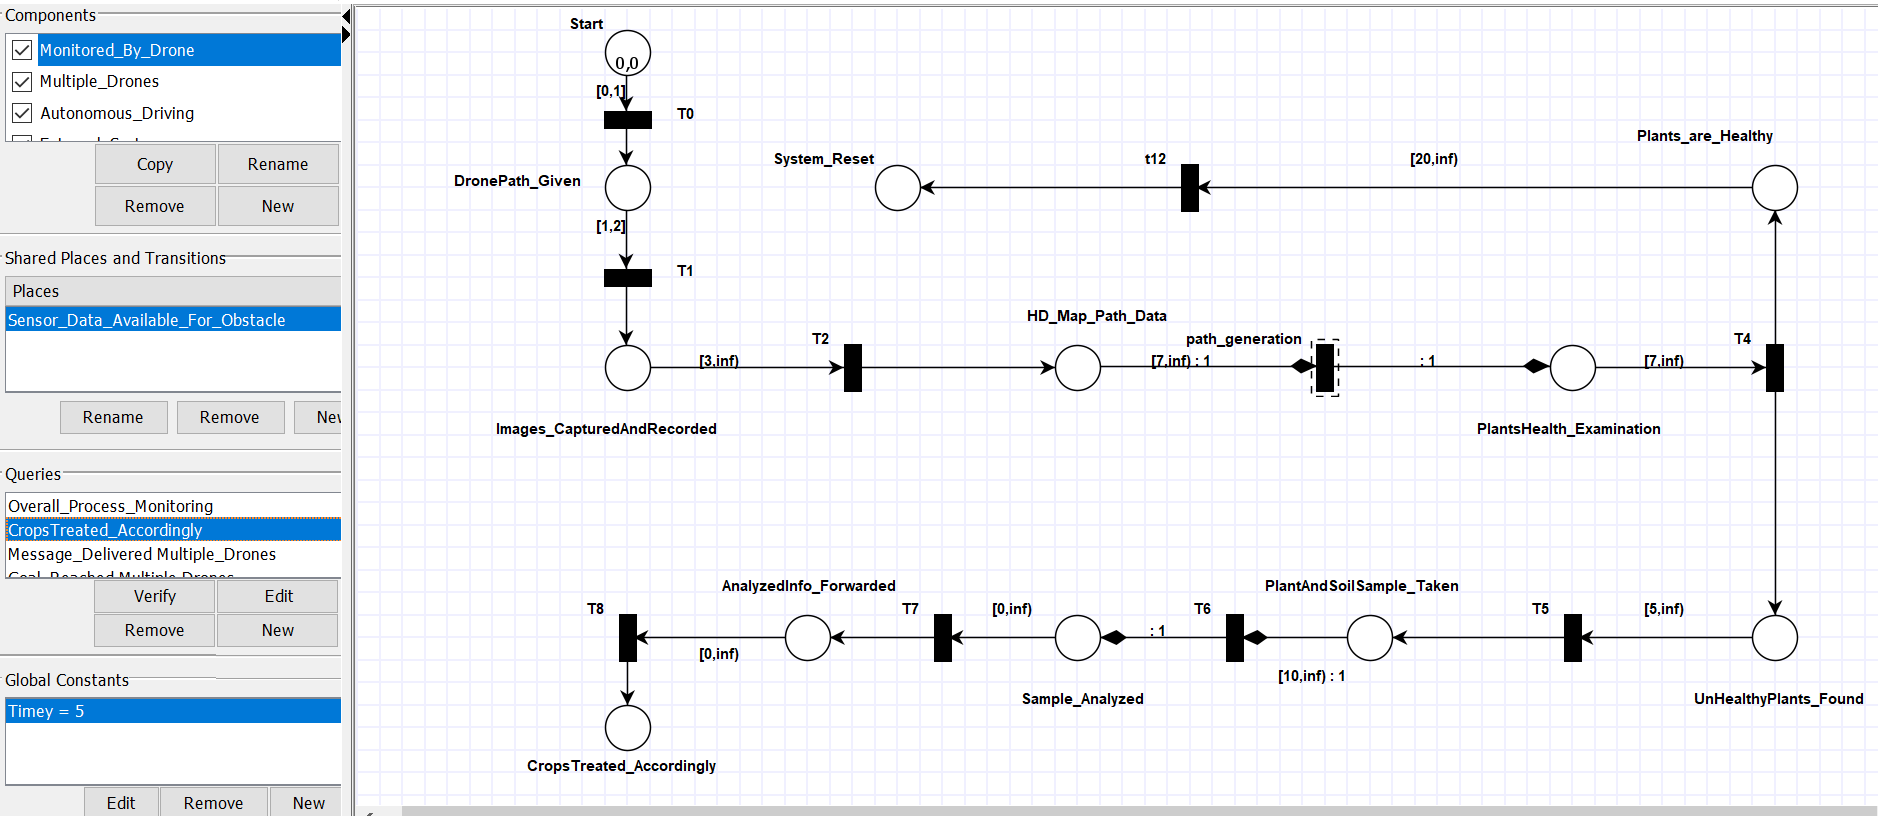
\includegraphics[width=1\textwidth]{Template/fig/Tapaal model.png}
    \centering
    \caption{Modelling and Verification of Monitoring by Drone}
\end{figure}

Now, the farmer will look into that map details generated by the internal system in order to observe plants’ health. We can see that there are two cases after this place in our model; one case will be considered when no unhealthy plant is found then our system will reset and the process can restart whenever it is desired, the second case will be considered when the farmer finds unhealthy plants in that specific area of the field. As the unhealthy plants are found, the farmer and agronomist will scout and collect plant and soil sample from those areas where there are unhealthy plants. The agronomist will then analyze the problem through those samples in lab. Once, the samples are analyzed, the agronomist will share the analyzed information with the farmer and the farmer will then treat the crops accordingly. 

\subsection{TAPAAL Model of Autonomous farming Vehicles (Moaz)}
In the TAPAAL model of this scenario various places and transitions are involved, some of which are shared and some are standalone that execute on their own.  As the scenario begins the motor of the farming vehicle is turned on, simultaneously the vehicle tries to establish a connection with the Drones present in the field and the farming Scientist so that autonomous ability of the farming vehicle can be enabled. Once the autonomous mobility feature is enabled the vehicle waits for the \textbf{HD-Map-Data} produced by the Routing-drones which are  capturing real time images which in turn is producing the path on which the farming vehicle is going to move. This particular transition in the model is shared with another scenario ''Monitored by drone'' in the system.\par
As the vehicle begins to move on the allocated map it now moves to carry out the harvesting operation. In the pathway if it encounters any obstacle at this stage it starts executing its obstacle-avoidance-manoeuvre which in this scenario is to wait for pre-defined time units present in the sensor data that is available on all possible obstacles in the field. As this is a shared place this information also comes from Operational-drones which are updating in real time. It then moves  to the next place \textbf{''Obstacle-avoided''}  and then converges back to the normal transition of new path allocation. After this transition normal Farming operation is carried out and an output report is sent to initial Communication-place for the report building of the current progress of the field. This whole system is modelled in Figure 9.
\begin{figure}
    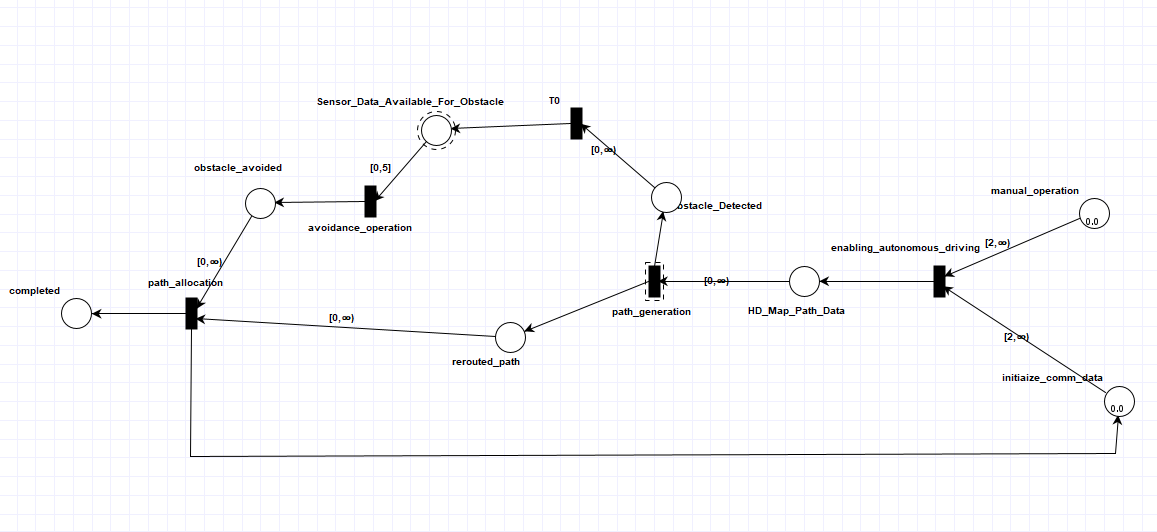
\includegraphics[width=1\textwidth]{Template/fig/AfV.png}
    \centering
    \caption{Modelling and Verification of Autonomous Farming Vehicles}
\end{figure}

\subsection{Tapaal: Multiple Drones (Tunde Oluwayemi Aluko)}
\begin{figure}[htp]
    \centering
    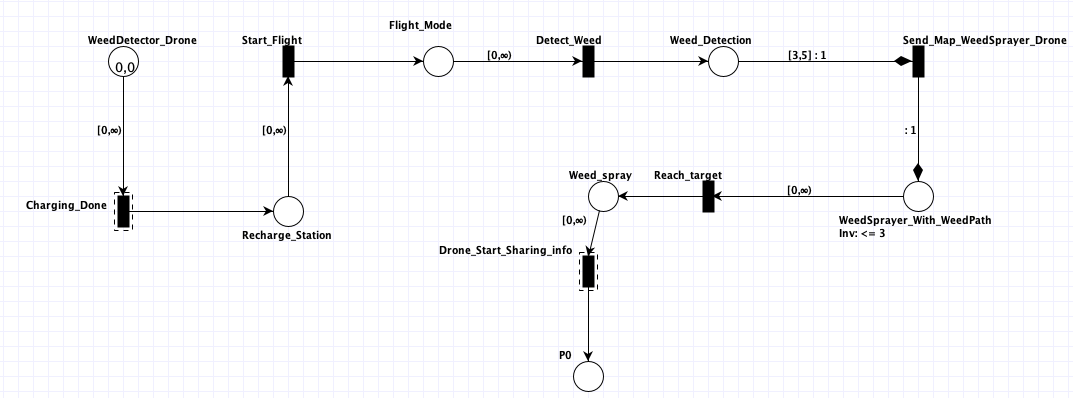
\includegraphics[width=8cm]{Template/fig/Multiple_Model.png}
    \caption{Modelling of multiple drones TAPAAL}
    \label{fig:mutile_mod}
\end{figure}

We model our use-case diagram in TAPAAl as seen in figure \ref{fig:multilpe_drones}. The weed detector drone first goes to the charging station; after the charging is done, flight mode is activated and starts flying over the farmland to detect weed. Once the weed is detected, the weed detector drone sends the weed path to the weed sprayer drone within three to five-time units. The rest of the model is self-explanatory. We then tried to verify some part of the model, too, as seen in figure \ref{fig:multiVer}, and the overall verification was satisfied.

\begin{figure}[htp]
    \centering
    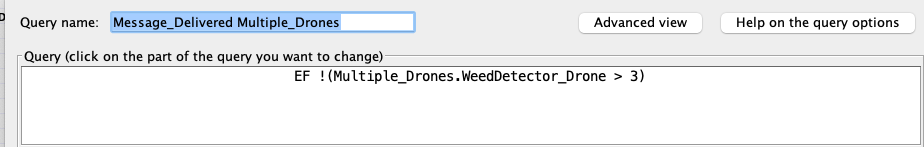
\includegraphics[width=5cm]{Template/fig/verification_multiple.png}
    \caption{Verification of Weed Detector in TAPAAL}
    \label{fig:multiVer}
\end{figure}
\section{Deep Learning Approach for Precision Farming (Tunde Oluwayemi Aluko)}

The Deep Learning algorithm excels in recognizing patterns in enormous amounts of data. Object recognition from images is accomplished utilizing three or more layers of artificial neural networks, each extracting many features.

In this project, we have used fastai as our framework and Jyputer Notebook as the environment for training our training. The GPU server configuration is as follow:
\begin{itemize}
    \item[] GPU: NVIDIA-SMI 
    \item[] Version: 460.106.00   
    \item[] Driver Version: 460.106.00   
    \item[] CUDA Version: 11.2  
\end{itemize}

This section will describe the dataset we used, the algorithm, analysis of our training and the result.

\subsection{Dataset  (Fawad Murad)}

In deep learning approach, the first and most essential thing was to build a dataset on which the training of our system was based. Images of 12 known types of plant; 'black grass', 'charlock', 'cleavers', 'common chickweed', 'common wheat', 'fat hen', 'loose silky bent', 'maize', 'scentless mayweed', 'shepherds purse', 'small flowered cranesbill' and 'sugar beet' were supposed to be present in dataset. Even though, a collective data of these types of plant is already available in the given Jupyter notebook but we collected our own data from different sources by using different tools, like Python library, Kaggle, directly from Google images, etc. 

First, we downloaded images individually as the collection of 900 images was distributed among four members. There were also few inefficient images among the whole collection of data we downloaded in bulk, so we had to double-check every image in order to observe its quality. We named each image file from 000 to 899 after gathering the data. Then, we created a CSV file in which semicolon (;) was used as a separator. The headers id and label appear in the first row (id;label), the second row has the number 000 and the label (000;black grass) and the 001 and the accompanying label (001;fat hen) are in the third row, and so on. The flight paths of all drones were also logged in a CSV file and one file was assigned for one drone. For example, each file contains the squares that the drone travels through (000;001;002;003;004). In the end, the dataset was uploaded as single zip file named with group name.


\subsection{Algorithm (Tunde Oluwayemi Aluko)}
Figure \ref{fig:deepLalg} shows our approach to weed detection using a deep learning algorithm. First, our drone detects the object and uses the CNN algorithm to classify the plant as a weed or some other plant. We would further describe this concept a bit further. 
\begin{figure}[htp]
    \centering
    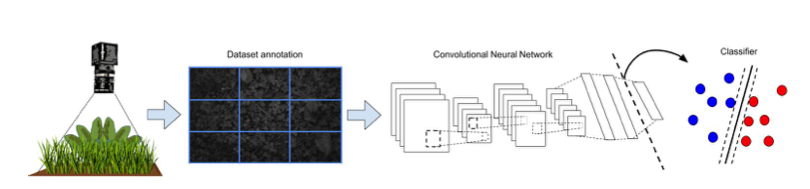
\includegraphics[width=10cm]{Template/fig/deepl_approach.png}
    \caption{Deep Learning based approach to weed recognition\cite{kounalakis2019deep}}
    \label{fig:deepLalg}
\end{figure}

\emph{Convolution Neural Network (CNN)} has layers such as Convolution, ReLU Layer, Pooling, Fully Connected, and others. This model works in the same way as neurons in the human brain, with each neuron taking an input, doing some action, and then passing the results to the subsequent neurons. The images would be compared piece by piece using CNN. 
CNN compares images piece by piece using a feature-based algorithm. CNN employs the weight matrix to extract specific features from the input image without losing information about the image's spatial organization.

\emph{Transfer learning} reduces the number of parameters in a model by applying a piece of the trained model on a familiar task in the new model. Transfer learning is a machine learning technique that uses a previously trained neural network. So, when we use the new model to analyze our original dataset, we effectively leverage the previously extracted features and train the model with our dataset. Furthermore, because the feature extraction phase does not need to be trained, we may train the model with minimal resources, datasets, and time\cite{hasan2019deep}.

We have used RestNet\cite{he2016deep}, a transfer learning model based on ImageNet\cite{deng2009imagenet} this project. 

\subsection{Analysis (Enkeledi Mema)}
After the deep learning algorithm implementation and model training,further analysis were done. In these analysis is included the wrong images classification. By identifying which images are classified wrong in a higher amount,it is possibles to perform further optimisation on the learner and training phase. If it is necessary, further pre-processing optimisation can be done on the data set. It was checked carefully the confusion matrix and other graphical information to find a suitable error rate and to decrease it. Our goal is to train our model in the best way. By analysing the confusion matrix carefully, it was noticeable a huge wrong classification of lose silky bent and black grass. Both plants in a young state were very similar and the model had difficulties in classifications. Therefore, we did optimization on the data set as well we performed more epochs and other data manipulation offered by fast-ai library and pytorch. Another function was used to make interpretation top losses. By analysing in details the function output, it was possible to check the prediction that was made ,what actually the image represents, the loss rate and what is the probability for a wrong classification. This was a really important tool to show visually the images that were classified wrong. Also to check the abilities that our model offers in image recognition and classification, we decided to take a random image from web. We tried to classify this image by using or model. In such kind of experiment we got relatively good result and the probability to receive a right classification was more than 90 percent.          


\subsection{Result/Prediction Moaz}
After the overall implementation of the whole data set final result that we achieved is shown in Figure 11. By using different architectures, we achieved different results. The best result was achieved by using \textbf{''restnet152''}. As the model became more familiar with the data set the overall accuracy rate in each epoch increased. After 15 successful epochs, we managed to get an accuracy of 94\% which is quite optimal considering we used a medium-sized data set that was compiled in a not-so-easy manner. 


\begin{figure}[h]
    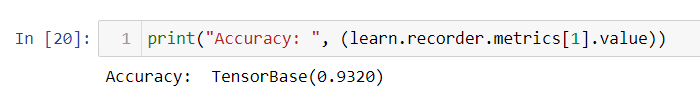
\includegraphics[width=.8\textwidth]{Template/fig/result.png}
    \centering
    \caption{Accuracy of our Model}
\end{figure}

\section{Conclusion Moaz}
At the beginning of this project, we started with an abstract and basic idea about farming. After moving to the specific scenario allocation whole project started to make sense as we all could come up with our Use-Cases. Then we developed specific use cases that suited each scenario. After our use-cases were solidified we modeled our use cases and then connected them simultaneously where each scenario was co-dependent on each other. At this stage, we used different verification techniques to check for various deadlocks and tried to come up with a solution that will be a final working solution for all our linked scenarios. In the end, by implementing deep learning in classifying different images and using different algorithms in differentiating between elements of various data sets we became more familiar with Python and its libraries as a whole. As this project involved using a modeling tool TAPAAL we also acquainted ourselves with various verification techniques. This project gave us a real-time idea about how actual ''Smart Farming'' in the industry is being executed. The overall experience of this whole project was really good for us all as it opened another door of knowledge about Precision Farming. We learned new methods in which farming which is the backbone of every food industry can revolutionize.


\begin{center}
\textbf{Declaration of Originality}
\end{center}

We, Tunde Oluwayemi Aluko, Enkeledi Mema, Fawad Murad, and Muhammad Moaz Amin herewith declare that we have composed the present paper and work by our self and without use of any other than the cited sources and aids. Sentences or parts of sentences quoted literally are marked as such; other references with regard to the statement and scope are indicated by full details of the publications concerned. The paper and work in the same or similar form has not been submitted to any examination body and has not been published. This paper was not yet, even in part, used in another examination or as a course performance. We agree that our work may be checked by a plagiarism checker. 


%%% Angabe der .bib-Datei (ohne Endung) / State .bib file (for BibTeX usage)
\bibliography{mybibfile} %\printbibliography if you use biblatex/Biber
\end{document}
